%%%%%%%%%%%%%%%%%%%%%%%%%%%%%%%%%%%%%%%%%
% Compact Academic CV
% LaTeX Template
% Version 2.0 (6/7/2019)
%
% This template originates from:
% https://www.LaTeXTemplates.com
%
% Authors:
% Dario Taraborelli (http://nitens.org/taraborelli/home)
% Vel (vel@LaTeXTemplates.com)
%
% License:
% CC BY-NC-SA 3.0 (http://creativecommons.org/licenses/by-nc-sa/3.0/)
%
%%%%%%%%%%%%%%%%%%%%%%%%%%%%%%%%%%%%%%%%%

%----------------------------------------------------------------------------------------
%	PACKAGES AND OTHER DOCUMENT CONFIGURATIONS
%----------------------------------------------------------------------------------------

\documentclass[11pt]{article} % Default document font size

%%%%%%%%%%%%%%%%%%%%%%%%%%%%%%%%%%%%%%%%%
% Compact Academic CV
% Structural Definitions
% Version 1.0 (6/7/2019)
%
% This template originates from:
% https://www.LaTeXTemplates.com
%
% Authors:
% Dario Taraborelli (http://nitens.org/taraborelli/home)
% Vel (vel@LaTeXTemplates.com)
%
% License:
% CC BY-NC-SA 3.0 (http://creativecommons.org/licenses/by-nc-sa/3.0/)
%
%%%%%%%%%%%%%%%%%%%%%%%%%%%%%%%%%%%%%%%%%

%----------------------------------------------------------------------------------------
%	REQUIRED PACKAGES AND MISC CONFIGURATIONS
%----------------------------------------------------------------------------------------

\usepackage{graphicx} % Required for including images

\setlength{\parindent}{0pt} % Stop paragraph indentation

%----------------------------------------------------------------------------------------
%	MARGINS
%----------------------------------------------------------------------------------------

\usepackage{geometry} % Required for adjusting page dimensions and margins

\geometry{
	paper=a4paper, % Paper size, change to letterpaper for US letter size
	top=3.25cm, % Top margin
	bottom=4cm, % Bottom margin
	left=2.5cm, % Left margin
	right=2cm, % Right margin
	headheight=0.75cm, % Header height
	footskip=1cm, % Space from the bottom margin to the baseline of the footer
	headsep=0.75cm, % Space from the top margin to the baseline of the header
	%showframe, % Uncomment to show how the type block is set on the page
}

%----------------------------------------------------------------------------------------
%	FONTS
%----------------------------------------------------------------------------------------

\usepackage[utf8]{inputenc} % Required for inputting international characters
\usepackage[T1]{fontenc} % Output font encoding for international characters

\usepackage[semibold]{ebgaramond} % Use the EB Garamond font with a reduced bold weight

%----------------------------------------------------------------------------------------
%	SECTION STYLING
%----------------------------------------------------------------------------------------

\usepackage{sectsty} % Allows changing the font options for sections in a document

\sectionfont{\fontsize{13.5pt}{18pt}\selectfont} % Set font options for sections
\subsectionfont{\mdseries\scshape\normalsize} % Set font options for subsections
\subsubsectionfont{\mdseries\upshape\bfseries\normalsize} % Set font options for subsubsections

%----------------------------------------------------------------------------------------
%	MARGIN YEARS
%----------------------------------------------------------------------------------------

\usepackage{marginnote} % Required to output text in the margin

\newcommand{\years}[1]{\marginnote{\scriptsize #1}} % New command for adding years to the margin
\renewcommand*{\raggedleftmarginnote}{} % Left-align the years in the margin
\setlength{\marginparsep}{-10pt} % Move the margin content closer to the text
\reversemarginpar % Margin text to be output into the left margin instead of the default right margin

%----------------------------------------------------------------------------------------
%	COLOURS
%----------------------------------------------------------------------------------------

\usepackage[usenames, dvipsnames]{xcolor} % Required for specifying colours by name

%----------------------------------------------------------------------------------------
%	LINKS
%----------------------------------------------------------------------------------------

\usepackage[bookmarks, colorlinks, breaklinks]{hyperref} % Required for links

% Set link colours
\hypersetup{
	linkcolor=blue,
	citecolor=blue,
	filecolor=black,
	urlcolor=MidnightBlue
}
 % Include the file specifying the document structure and styling

% Set PDF meta-information
\hypersetup{
	pdftitle={Alexandra Shikunova - Curriculum vitae},
	pdfauthor={Alexandra Shikunova}
}
\usepackage{hyperref}
\usepackage{graphicx}
\usepackage{wrapfig}
\graphicspath{ {./images/} }

%----------------------------------------------------------------------------------------

\begin{document}

%----------------------------------------------------------------------------------------
%	CONTACT AND GENERAL INFORMATION
%----------------------------------------------------------------------------------------

\begin{wrapfigure}{r}{0.25\textwidth} %this figure will be at the right
    \centering
    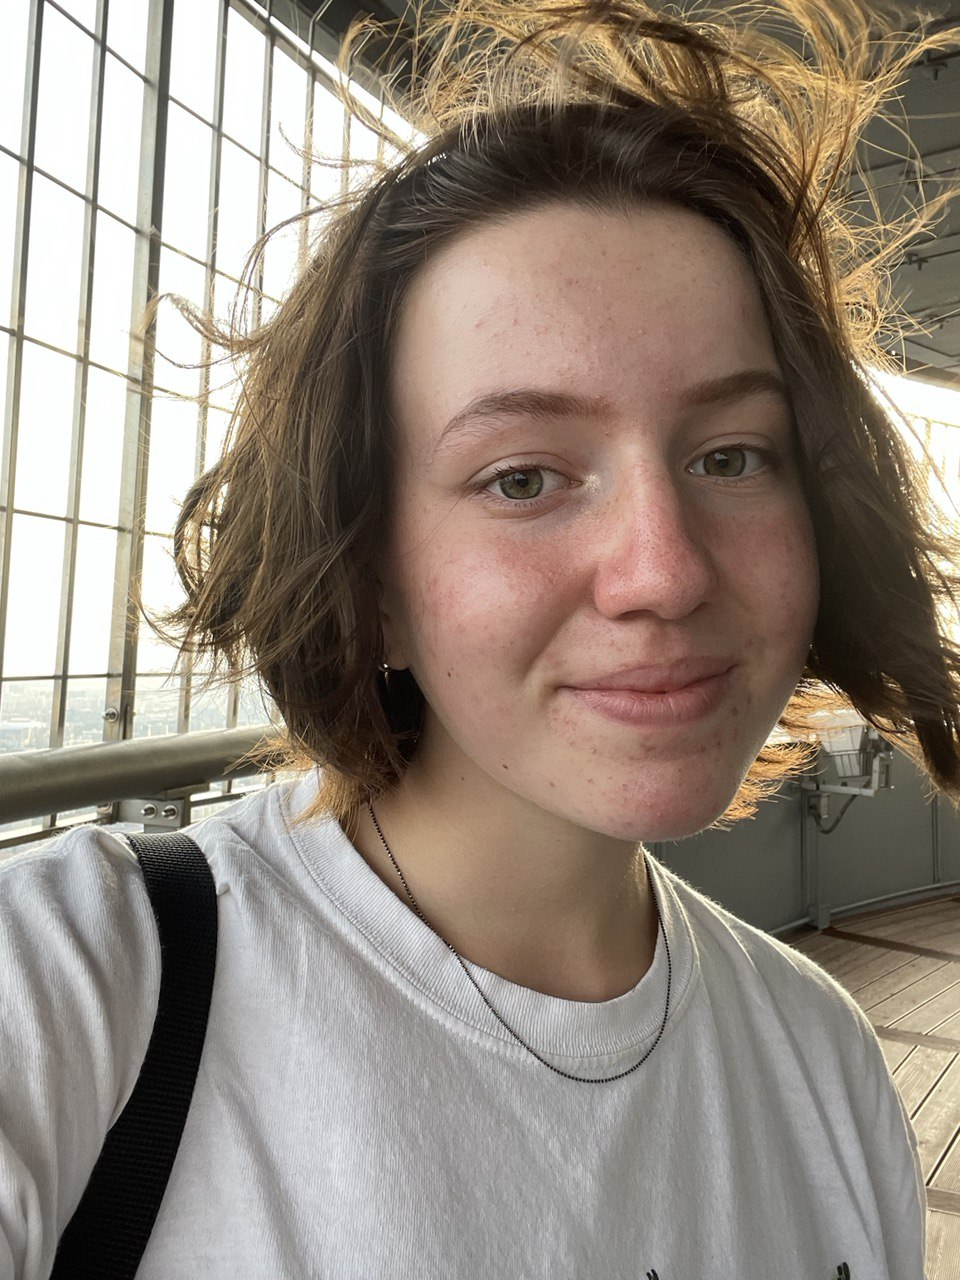
\includegraphics[width=0.25\textwidth]{photo}
\end{wrapfigure}
{\LARGE\bfseries Alexandra Shikunova} % Name
\bigskip\bigskip\medskip % Whitespace

Moscow, Russia\\
Born in 2002\\

\textit{Contacts:}\\
\textbf{\href{https://t.me/thnlgrlivrlvdwsbrnwthrssnhrys}{Telegram}}\\
\textbf{\href{mailto:notalexandrashikunova@gmail.com}{Email}}\\
\textbf{\href{https://github.com/poisongrapevine}{Github}}
\medskip % Whitespace

%------------------------------------------------

\section*{Skills and interests}

\textbf{Python, SQL, PySpark, Airflow, TeX, JavaScript (for PCIbex)}\\
\textbf{Interests}: machine learning, NLP, syntactic probing, MLOps

%----------------------------------------------------------------------------------------
%	EDUCATION
%----------------------------------------------------------------------------------------

\section*{Education}

\years{2021-2023} Data science minor, Faculty of computer science, HSE University, Moscow\\
\years{2020-2024} Computational linguistics major, Faculty of humanities, HSE University, Moscow

%----------------------------------------------------------------------------------------
%	WORK EXPERIENCE
%----------------------------------------------------------------------------------------

\section*{Work experience}

\years{since 2023} \textbf{NLP engineer at Sberbank}\\
\years{since 2021} \textbf{Research assistant at HSE Laboratory in Formal Models in Linguistics}\\
\years{since 2020} \textbf{Private tutoring in English as a foreign language}\\
\years{2022} Teaching assistant in Python for data science minor, HSE\\
\years{2022-2023} Data scentist, NLP team, Megafon\\
\years{2022} {Machine learning \& big data intern, NLP team, Megafon}\\
\years{2021}Teaching assistant in discrete mathematics

%\section*{Доклады и публикации}

%\years{доклад} \textbf{ТМП 2022} Idioms, NP position and control: evidence from Russian (в соавторстве с Павлом Рудневым)\\
%\years{доклад} \textbf{SOUL 4} Case and agreement puzzle in the Moksha debitive\\
%\years{постер, статья} \textbf{ConSOLE 30} Mermaid construction: a case of Kazym Khanty\\

\section*{Pet projects}

\years{2022}\href{https://github.com/thddbptnsndshs/LMindbiases}{Investigating inductive biases in language models} (pytorch, spacy)\\
\years{2022}\href{https://github.com/thddbptnsndshs/motustoday}{Infographics for the Motus database of migrating animals} (sql, sklearn, Flask)\\
\years{2021}\href{https://github.com/thddbptnsndshs/idioms}{Statistical analysis of experimental data with Python} (sklearn)\\
\years{2021}\href{https://github.com/thddbptnsndshs/nlzlkskprdstvtljsclnhgrppncnvfrmvgrppvk}{Telegram bot for orthography checking of VK groups} (Telegram/VK API)\\

\section*{Languages}

\textbf{Russian} native\\
\textbf{English} proficient\\
\textbf{German, Persian, Polish} beginner


%----------------------------------------------------------------------------------------
%	FINAL FOOTER
%----------------------------------------------------------------------------------------

% Any final footer text such as a URL to the latest version of this CV, last updated date, compiled in XeTeX, etc

%----------------------------------------------------------------------------------------

\end{document}
